\section{Diseño de Interfaces}
\label{sec:diseno_interfaces}

El diseño de interfaces considera dos aplicaciones: el portal VlmHub, orientado a la administración del procesamiento documental, y el Buscador Avanzado de Documentos, destinado a consultar el contenido transcrito e indexado.

\subsection{Modelo de Navegación}
\label{subsec:modelo_navegacion}

VlmHub utiliza una navegación jerárquica protegida por autenticación. Desde la vista de ingreso se accede a la página principal, que permite consultar el estado de los servicios y elegir entre la administración de tareas y la creación de un nuevo procesamiento. El flujo de procesamiento guía al usuario por la selección de la fuente documental, la configuración del lote y la confirmación de la tarea. Desde la lista de tareas se puede acceder al detalle, progreso, resultados y errores de cada ejecución.

\begin{figure}[htbp]
    \centering
    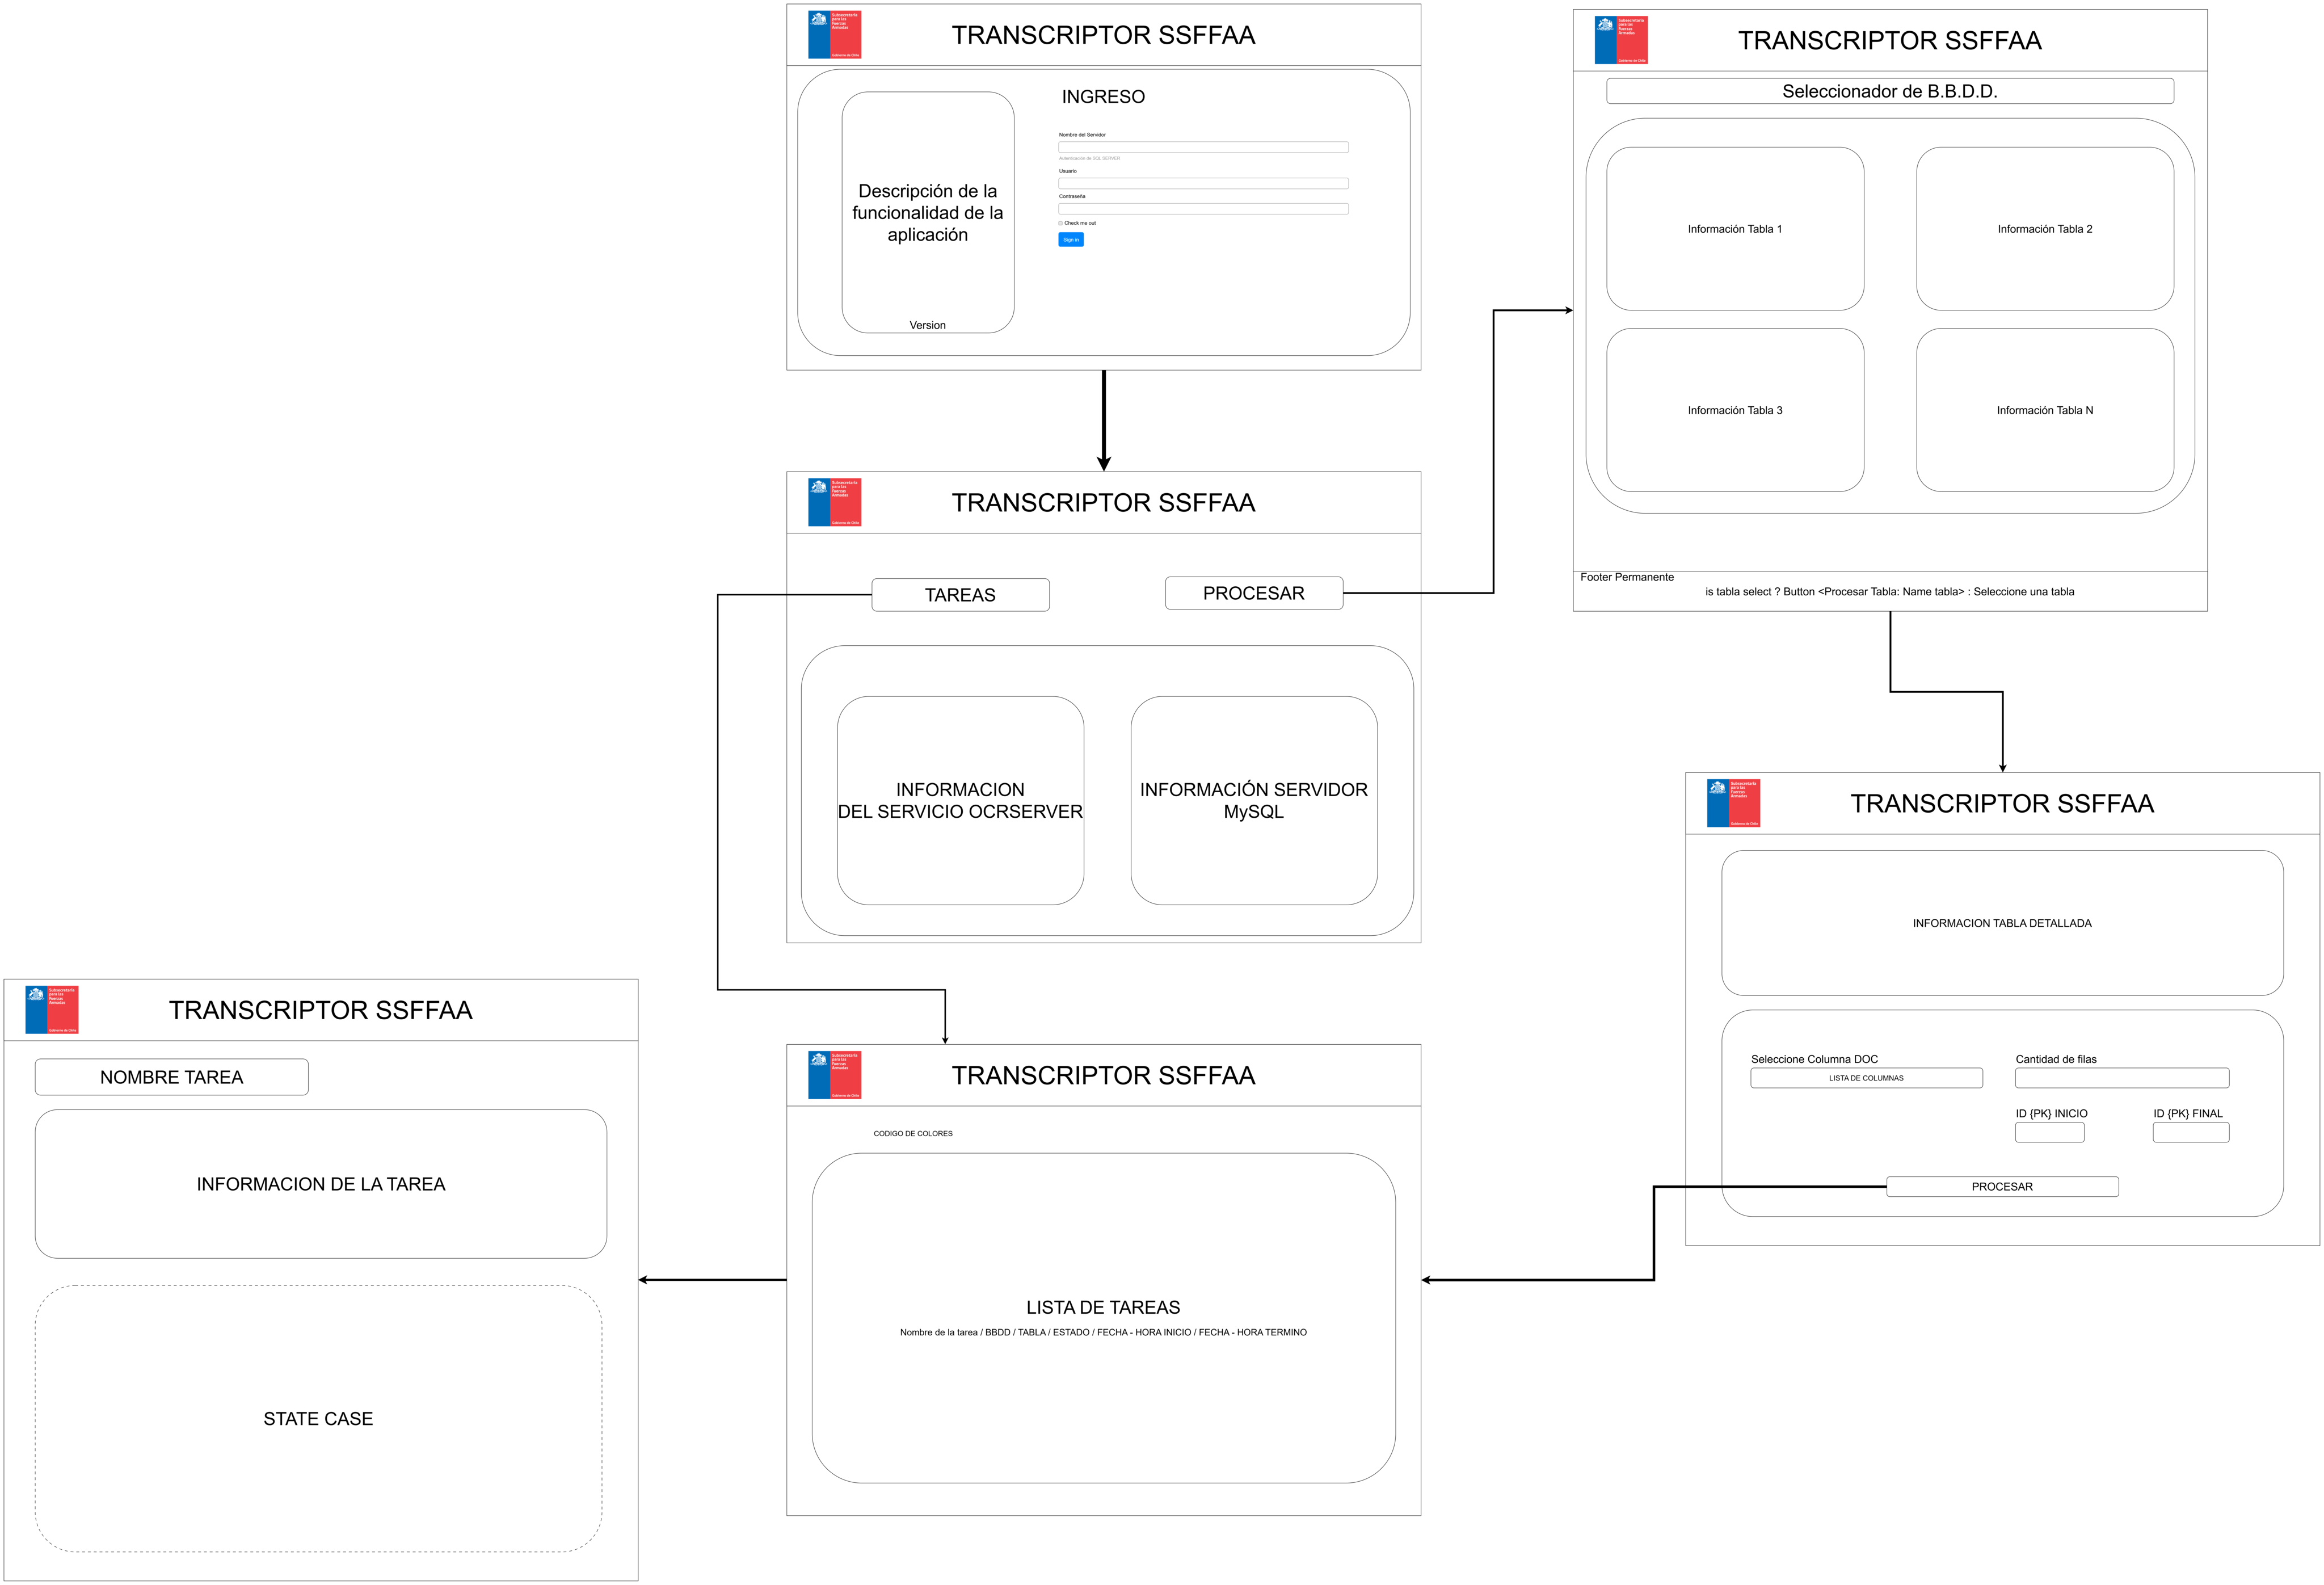
\includegraphics[width=\linewidth]{images/Interfaz_VlmHub.png}
    \caption{Modelo de vistas y navegación de VlmHub.}
    \label{fig:modelo_navegacion_vlmhub}
\end{figure}

El Buscador Avanzado mantiene un flujo independiente y directo: el usuario ingresa una consulta, aplica filtros o selecciona un perfil de búsqueda, revisa los resultados paginados y abre el documento en la página donde se encontró la coincidencia. La navegación permite regresar a los resultados sin perder la consulta ni los filtros aplicados.

\subsection{Diseño de Interfaces Usuarias}
\label{subsec:diseno_interfaces_usuarias}

\begin{figure}[htbp]
    \centering
    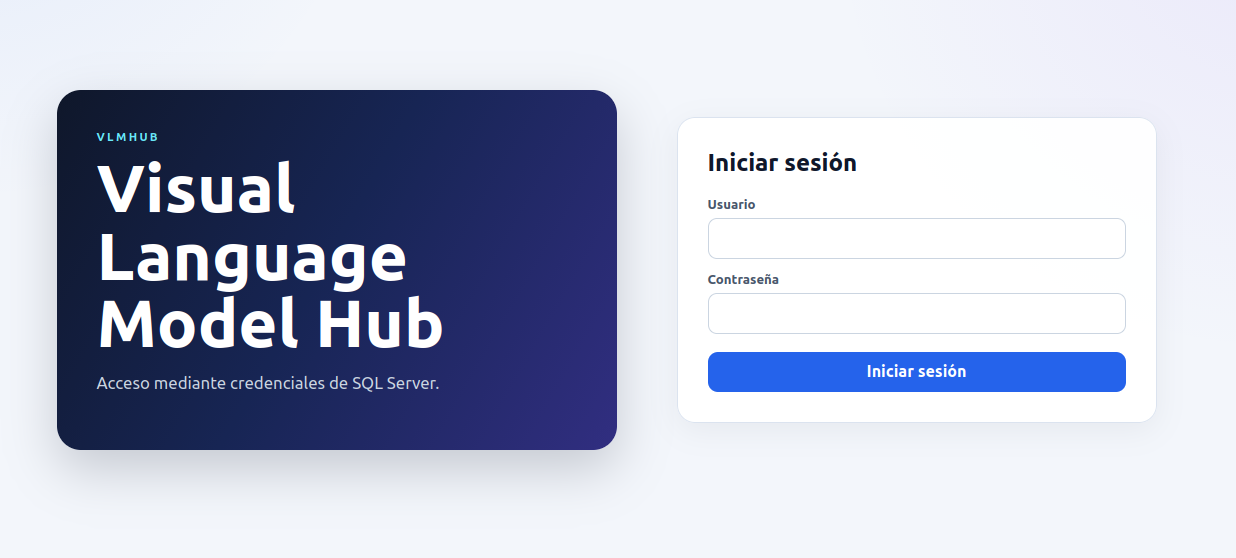
\includegraphics[width=0.7\linewidth]{images/loginVlmHub.png}
    \caption{Interfaz usuaria de VlmHub.}
    \label{fig:interfaz_vlmhub}
\end{figure}

\begin{figure}[htbp]
    \centering
    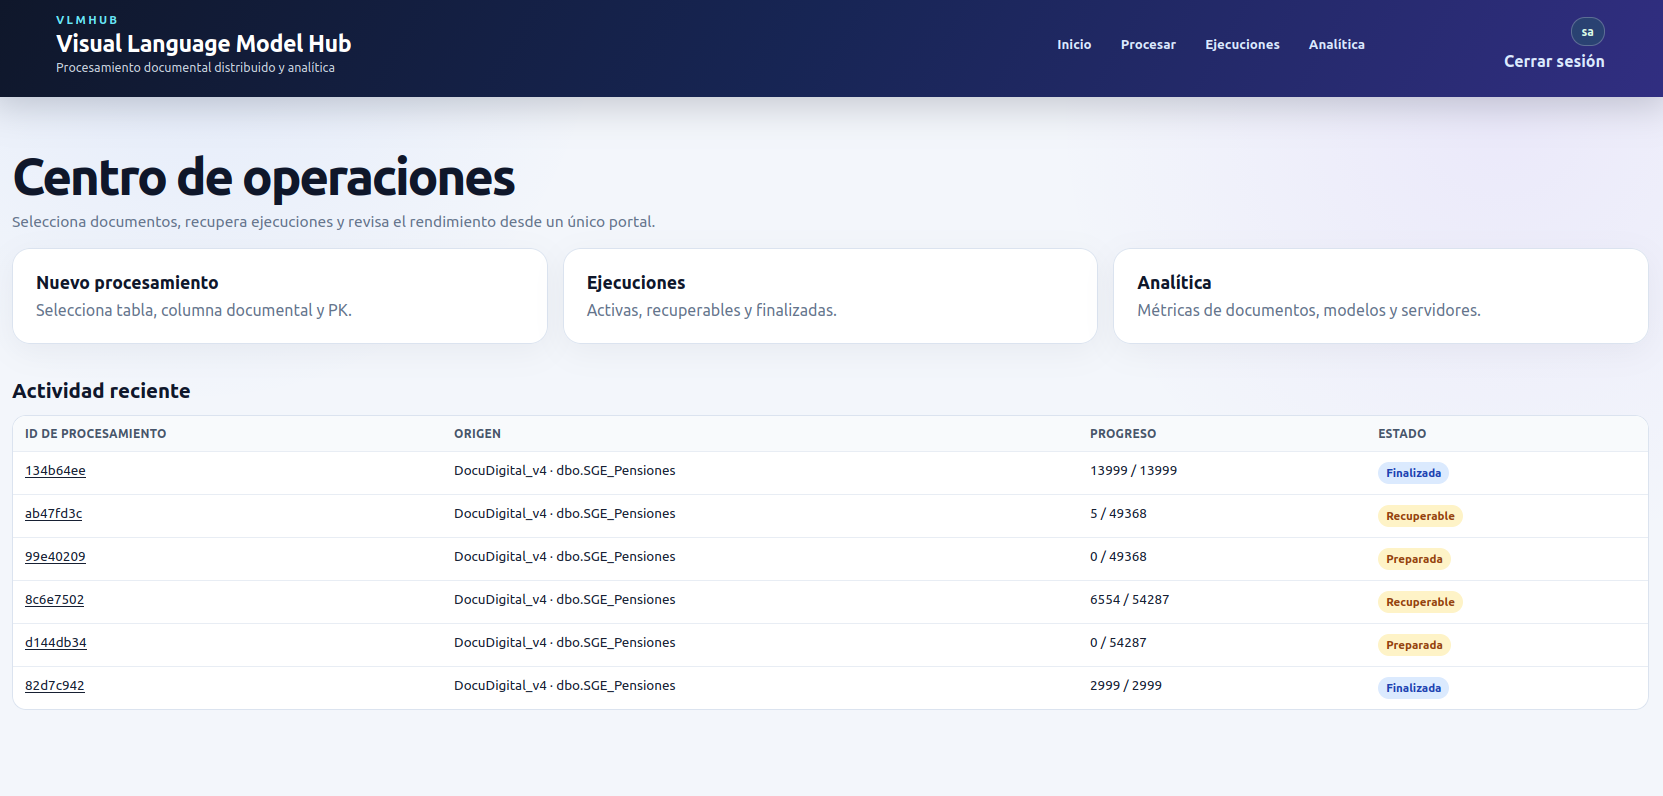
\includegraphics[width=0.7\linewidth]{images/menuVlmHub.png}
    \caption{Interfaz usuaria de VlmHub.}
    \label{fig:interfaz_vlmhub}
\end{figure}

La interfaz de VlmHub se organiza en vistas de ingreso, estado general, preparación de lotes, lista de tareas y detalle de tarea. Los formularios deben identificar los campos obligatorios, validar los parámetros antes del envío y evitar solicitudes duplicadas. Los estados de procesamiento deben distinguir visualmente tareas pendientes, en ejecución, completadas, canceladas y fallidas, mostrando el avance y los antecedentes necesarios para revisar un error.

\begin{figure}[htbp]
    \centering
    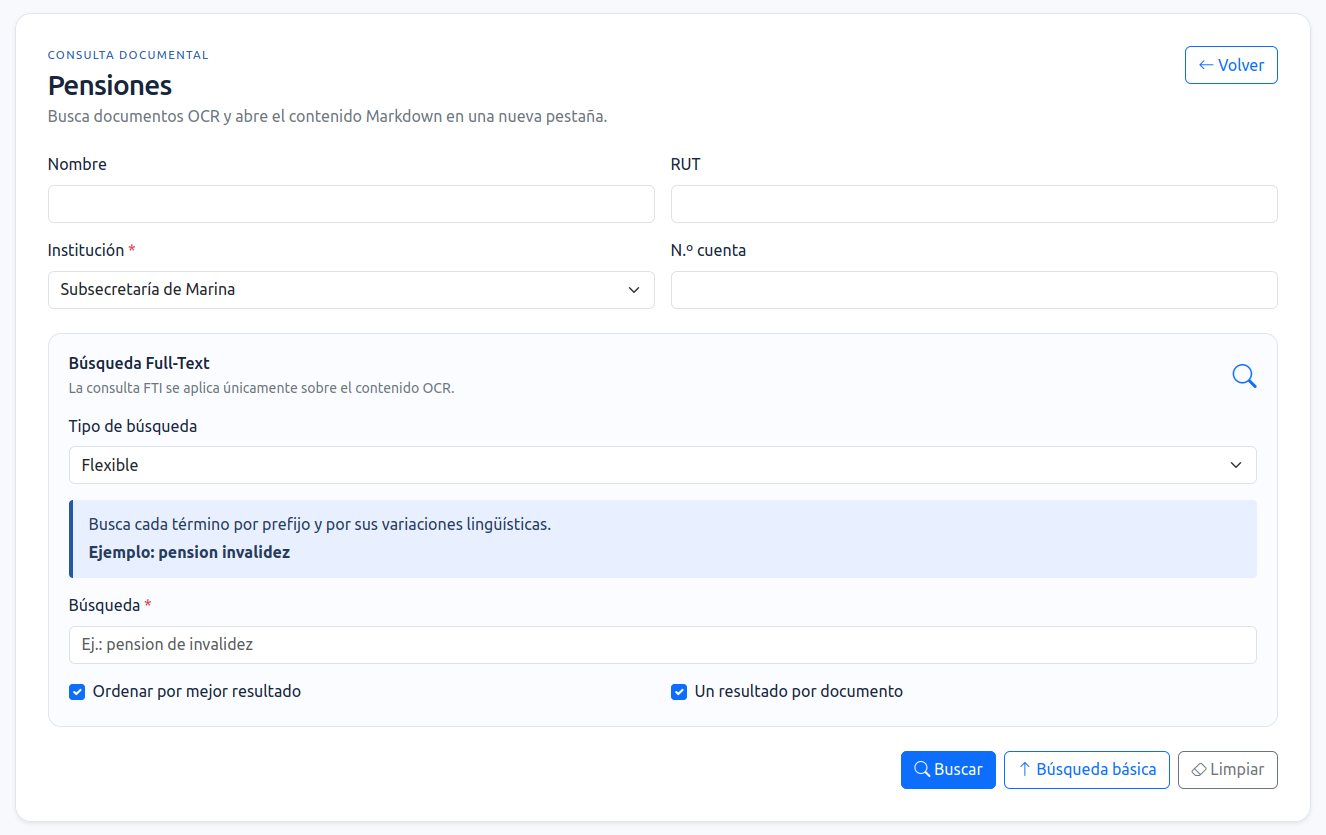
\includegraphics[width=0.7\linewidth]{images/BusquedaAvanzada.png}
    \caption{Interfaz usuaria del Buscador Avanzado de Documentos.}
    \label{fig:interfaz_buscador}
\end{figure}

La interfaz del Buscador Avanzado debe disponer de un campo de consulta principal, filtros por metadatos, perfiles de precisión y controles de paginación. Cada resultado debe mostrar su relevancia, un fragmento de contexto, los metadatos autorizados y la página correspondiente, además de una acción para abrir el documento original. Las coincidencias exactas, especialmente identificadores, deben diferenciarse de las aproximadas.
    
        